\chapter{Data and Methodology}
This chapter outlines the~data collection framework and the~implementation of \gls{nlp} and machine learning model. The~data pipeline begins with the~automated scraping and text processing of the~\gls{ecb}'s monetary policy statement transcripts. The~extracted and processed text is located into a~custom \textit{SQLite} database. In this database we include sentiment and topic metadata, which are formed by \textit{BERT} familiar models and zero-shot topic classifier. This architecture ensures data integrity and provides a~robust foundation for subsequent macroeconomic and market variables interaction modeling.

\section{Data Scraping and Preprocessing}
Datasets of \gls{ecb} communications are publicly available. Nonetheless, for fine-grained sentiment analysis, they lack the~neccessary level of detail. Moreover, most sources provide uniform text blocks without distinguishing between the~\gls{is} and \gls{qa} components. Our decision to develop a~custom scraping pipeline was driven by the~need to isolate the~responses of \gls{ecb} officials from the~questions posed by journalists. This allowed for a~more precise extraction of \gls{mp} signals, which are free from the~sentiment bias caused by journalistic questioning. The~first phase focuses on the~preparation of a~dataset of transcripts from \gls{gc} conferences. This preparation is divided into two primary tasks. The~first task involves the~retrieval of hyperlinks to scrape webpages, while the~second focuses on parsing the~content into two logical segments and storing these parts in a~robust, structured format.

The~scraping pipeline initially retrieves the~raw \textit{HTML} pages and extracts the~relevant textual content. To accurately separate the~\gls{is} from the~\gls{qa} session, the~pipeline utilizes custom Regular Expressions (Regex). After initial investigation, we defined specific structural markers in the~transcripts the~algorithm precisely splits the~document. These markers included phrases such as \textbf{``My first question...''} or \textbf{``Transcript of the~questions''}. Furthermore, within the~\gls{qa} segments, the~script distinguishes the~responses of \gls{ecb} officials from the~journalists' questions. The~raw extracted data, including dates and URLs, are temporarily stored in a~Pipe-Separated Values (.psv) format.

% Samotný diagram
\begin{figure}[ht]
    \centering
    \begin{tikzpicture}[node distance=1.2cm and 1.5cm] % Vertikálna a~horizontálna medzera

        % Prvé tri idú doprava
        \node (start) [startstop] {URL Extraction \\ \footnotesize (Iterative loop)};
        \node (parse) [process, right=of start] {HTML Parsing \\ \footnotesize (BeautifulSoup)};
        \node (bifurc) [process, right=of parse] {Bifurcation \\ \footnotesize (Intro vs. \gls{qa} split)};

        % Štvrtý ide DOLE pod tretí
        \node (norm) [process, below=of bifurc] {Normalization \\ \footnotesize (Bold/italic handling)};

        % Piaty ide DOĽAVA od štvrtého (pod druhý)
        \node (stop) [startstop, left=of norm, fill=green!20] {PSV File};

        % Prepojenia (Arrows)
        \draw [arrow] (start) -- (parse);
        \draw [arrow] (parse) -- (bifurc);
        \draw [arrow] (bifurc) -- (norm);
        \draw [arrow] (norm) -- (stop);

    \end{tikzpicture}
    \caption{The~Data Acquisition and Preprocessing Pipeline}
    \label{fig:data_pipeline_snake}
\end{figure}

\subsection{Iterative Extraction of ECB Discourse}

Before the~text extraction from the~transcript of the~press conference, the~acquisition of the~hyperlink list was required. The~entire acquisition pipeline is visualized in Figure \ref{fig:data_pipeline_snake}. To acquire a~complete list of meeting URLs, the~\textit{HTML} source of the~official \href{https://www.ecb.europa.eu/press/press_conference/monetary-policy-statement/html/index.en.html}{ECB monetary policy statement list} was analyzed. The~primary index page is interactive and necessitates scrolling to load every hyperlink. Therefore, we needed the~implementation of a~\textit{Selenium WebDriver} for browser automation. However, we discovered a~more algorithmically efficient alternative. We managed to retrieve the~backend structure with year-specific placeholders: \nolinkurl{https:// www.ecb.europa.eu/press/press\_conference/monetary-policy-statement/{year}/ html/index\_include.en.html}.

Hence, we applied the~iterative loop across all relevant years. This streamlines the~hypertext link extraction process by avoiding browser interactions. This process, spanning from the~\gls{ecb}'s establishment to the~present, yielded a~total of $291$ unique transcripts.

\subsection{Content Parsing and Data Structuring}

The~link provides access to the~\gls{mps}, which is described in greater detail in Section \ref{subsection:mps}. Text extraction from the~\gls{mps}
encountered visually organized yet, within the~underlying \textit{HTML} hierarchy, unsystematic \textit{HTML} code. We had to address an itemized list, which protrudes from the~main section; paragraphs and headings, which are enumerated below. Furthermore, the~\gls{qa} section is not separated from the~ introductory statement by any \textit{HTML} tag. Consequently, the~heuristic approach, combining conditional logic with regular expressions, executes the~bifurcation of the~document into logical parts.

Both parts are segmented into paragraphs, with each paragraph designed to address a~single subject. Consequently, the~paragraph functions as an~atomic component. Therefore, questions and answers do not coexist in the~same paragraph in the~\gls{qa} section. For this reason \textit{HTML} content is parsed and stored in a~Pipe-Separated Values (PSV) file. This format was specifically chosen to prevent delimiter collisions with the~punctuation utilized by the~\gls{ecb} discourse. The~resulting dataset consists of five primary features: \textbf{statement\_id} (unique identifier), \textbf{date}, \textbf{url}, \textbf{intro} (the~prepared introductory statement), and \textbf{qa} (the~unscripted dialogue).

To preserve the~internal structure of the~paragraphs, both \textit{intro} and \textit{qa} columns are tab-delimited for paragraph separation. The~column containing the~\gls{qa} segment has an~extra feature: square brackets to maintain italic or bold style. These styles are utilized in the~\gls{qa} section to distinguish a~journalist's question and a~president's answer. As visualized in Figure \ref{fig:qa.styling}, questions are bold or italic, while answers are plain text. However, this structure is not universally applied; certain \gls{qa} segments are instead prefixed with identifiers such as \{question:\} or the~speaker's name, followed by unformatted text.

\begin{figure}[ht]
    \centering
    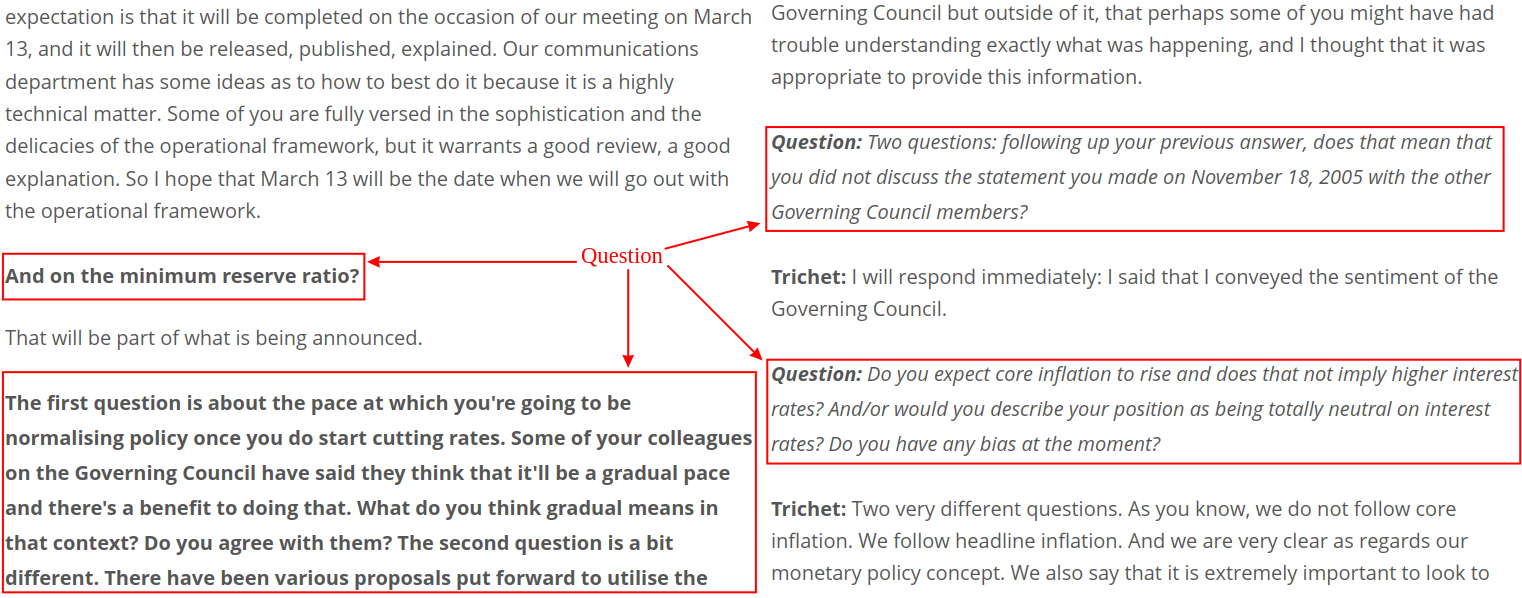
\includegraphics[width=1\linewidth]{images/data/qa_example_of_style.png}
    \caption[Evolution of formatting styles in ECB transcripts]{\centering Evolution of formatting styles in ECB transcripts. The~2005 transcript
        (right) utilizes explicit speaker labels, whereas the~2024 version (left) relies on font styling (bold/italic) to distinguish between
        speakers.}
    \label{fig:qa.styling}
\end{figure}

\section{Quantifying Central Bank Communications}
The~transition from qualitative narratives to quantitative market predictors requires a~systematic transformation of the~raw textual data. This stage of the~methodology is concerned with the~transformation of the~previous structured base dataset into a~more refined analytical collection. For this we use a~pipeline that reduces noise, considers limitations of models and adds metadata to the~text.

The~output of this pipeline is split into two specialized datasets that describe the~\gls{is} and \gls{qa} components. The~pipeline identifies themes through topic modelling. Moreover, it measures the~emotional tone of each observation via sentiment analysis. Unique identifiers are used to track the~original order of segments. This sustains the~chronological and contextual integrity of the~discourse. Binary classification is applied to the~\gls{qa} dataset to separate journalistic inquiries from official responses. This ensures the~analysis focuses on signals from\gls{ecb} officials.

\subsection{Text Segmentation and Contextual Windowing}

Further analysis requires strict rules, which enhance model behavior. By analyzing lengths and list of the~smallest paragraphs, we set the~minimum length of a~paragraph to $100$ characters. In this list, we observed redundant paragraphs, examples of which are provided in Table\ref{tab:redundant}. These passages are contextually sparse for transformers to identify the~sentiment or the~topic. Moreover, they do not hold valuable information for the~market audience.

\begin{table}[ht]
    \centering
    TODO doplniť reálne veci do tabuľky
    % v tabulke sa popis zvykne davat nad tabulku
    \caption{Illustrative examples of noisy paragraphs excluded from the~dataset.}
    %id tabulky
    \label{tab:redundant}
    % tu zacina samotna tabulka
    \begin{tabular}{@{}lr@{}}
        \toprule
        Paragraph content                                           & Character count \\ \midrule
        ``Thank you very much.''                                    & 21              \\
        ``I now leave the~floor to the~Vice-President.''            & 45              \\
        ``Question: Could you elaborate on the~inflation outlook?'' & 58              \\ \bottomrule
    \end{tabular}
\end{table}

Apart from this noise reduction, paragraph lengths often reach a~transformer’s token constraint, which is $512$ tokens per input for BERT-based models, including FinBERT and CentralBankRoBERTa. To address this, long paragraphs are processed into segments with an upper bound of $200$ words. This processing starts by partitioning passages into sentences using the~\textit{nltk.tokenize} library, which handles abbreviations and punctuation more robustly than simple splitting rules. The~preservation of full sentences is necessary for the~model's correct insight into the~context and syntactical structure of the~passage.

Our implementation follows an iterative approach where sentences are merged into a~segment until the~addition of the~next sentence would exceed the~maximum size. At that point, the~segment is closed, and a~new one is formed. Finally, for the~remaining text, we examine the~length of the~last segment of each paragraph. If this segment contains fewer than $30$ words, it is appended to the~preceding segment rather than being treated as an~independent input. This ensures that every segment processed by the~model contains sufficient semantic density, while the~combined length remains safely within the~transformer's token limitations.

Short paragraphs (that is, longer than $100$ characters but shorter than $30$ words) are maintained as independent segments. While shorter inputs may provide less context, their semantic integrity as independent statements or questions is considered more important for the~analysis than fulfilling a~word-count target. Finally, to ensure traceability, each segment retains the~metadata of its parent paragraph, including the~date, speaker identity, and section type (\gls{is} vs. \gls{qa}). This structure prevents the~``dilution'' of sentiment scores that occurs in excessively long text blocks and ensures that no segment is truncated. The~effectiveness of this segmentation and merging strategy is illustrated in Figure \ref{fig:distribution}, which compares the~word count distribution before and after the~transformation.

\begin{figure}[ht]
    \centering
    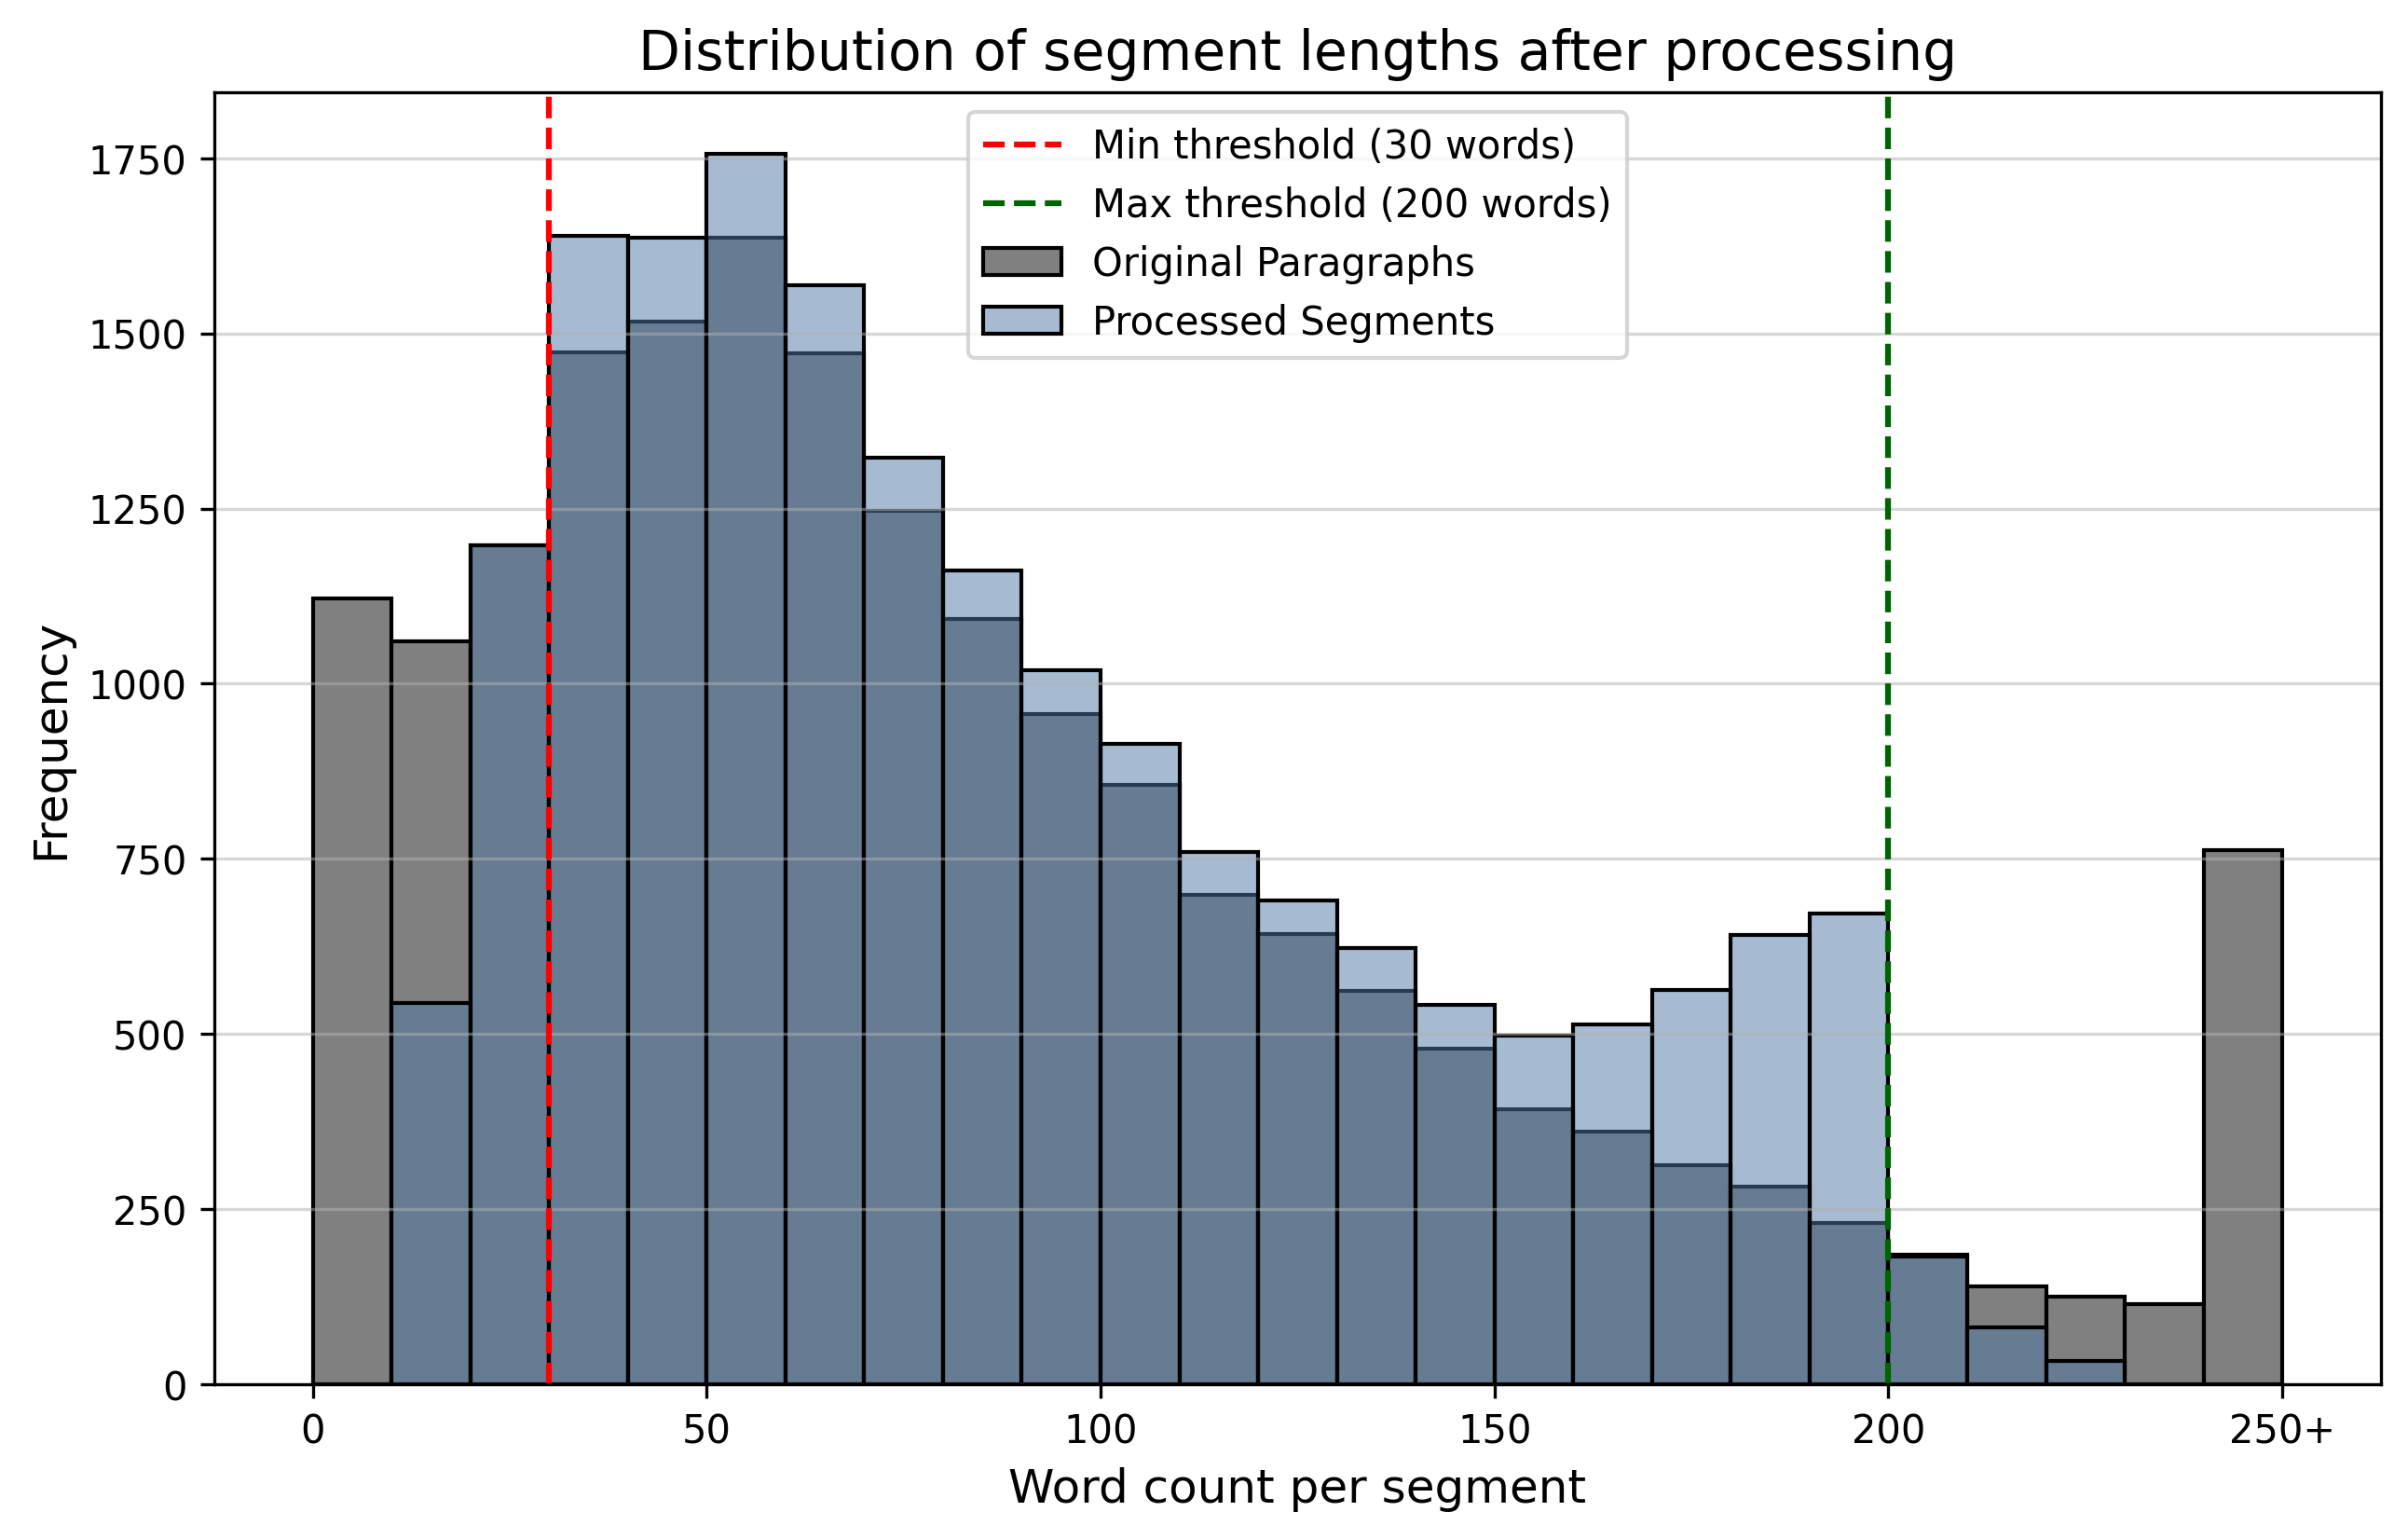
\includegraphics[width=1\linewidth]{images/data/segment_distribution.png}
    \caption[Impact of segmentation on text length distribution]{\centering Impact of segmentation on text length distribution. The~grey area
        represents original paragraphs with a~long tail of outliers, while the~blue area shows the~normalized segments adhering to the~$200$-word
        constraint.}
    \label{fig:distribution}
\end{figure}

\subsection{Zero-Shot Topic Classification}
While the~segments are now technically structured, they remain unlabelled raw text. To transform these strings into meaningful predictors, we must categorize them based on their thematic content. We considered several approaches to this task. Traditional Dictionary-based (Bag-of-Words) methods were dismissed due to their inability to capture context, such as negations or complex sentence patterns. Furthermore, training a~custom Topic modelling transformer on annotated data was not feasible given the~project’s time constraints and the~lack of a~pre-labelled domain-specific dataset.

Consequently, we decided to implement Zero-Shot Classification. This approach allows for the~classification of text into prescribed categories without requiring  explicit training on those specific labels. After reviewing current state-of-the-art models, we selected the~\textit{facebook/bart-large-mnli} model. This model is particularly suitable for our use case. Thus, it is pre-trained on Natural Language Inference (NLI) tasks. Further, it enables treating thematic labels as hypotheses to be tested against the~text segments.

We also started with a~list of ten detailed topics. This turned out to be a~mistake, because the~model suffered from a~sort of decision paralysis (much like a~human struggling to choose from a~massive menu). It became indecisive and ended up dumping almost everything into a~broad ``Risk Assessment'' category. To fix this, we radically simplified the~taxonomy to four core themes and replaced the~short titles with descriptive hypothesis strings. By narrowing the~choices and enriching the~context of each label, we forced the~model to be more certain. The~final set of labels and their descriptive strings are detailed in Table \ref{tab:labels}.
\begin{table}[ht]
    \centering
    \caption{Thematic labels and descriptive strings for Zero-Shot Classification}
    \label{tab:labels}
    \begin{tabular}{@{}lp{8cm}@{}}
        \toprule
        \textbf{Category}                & \textbf{Model Input (Label String)}                                            \\ \midrule
        Monetary Policy                  & ``inflation, price stability, interest rate decisions, monetary policy stance,
        financing conditions, bank lending, and market interest rates''                                                   \\ \addlinespace
        Economic Performance             & ``economic growth, GDP outlook, unemployment, labor market developments,
        macroeconomic risks, demand, consumption, and investment''                                                        \\ \addlinespace
        Fiscal             \& Structural & ``government budgets, national debt, public spending, and structural reforms'' \\ \addlinespace
        Other / Noise                    & ``general greetings, purely political questions, unrelated remarks, climate
        change, or personal comments (excluding macroeconomic impacts)''                                                  \\ \bottomrule
    \end{tabular}
\end{table}

The~``Other'' category is our final filter. It catches thematic noise. This noise includes politeness and procedural talk that doesn't actually move markets. By isolating these, we can later test if stripping away the~fluff actually sharpens our sentiment-based market predictions.

\subsection{Multi-Model Sentiment Extraction}
Once the~segments are labeled, the~next step involves extracting the~actual emotional tone (the~sentiment) from the~text. To ensure a~robust assessment, this research adopts a~parallel approach using two distinct architectures. This approach accounts for the~varying linguistic nuances captured by different model pre-training objectives. Therefore, we use a~two models paralleling approach (FinBERT and CentralBankRoBERTa) to evaluate every chunk in both the~\gls{is} and \gls{qa} datasets.

The~choice of these two models is intentional. FinBERT is the~industry standard for general financial text, while CentralBankRoBERTa is specifically tuned to recognize the~unique language of central bankers. It understands categories like ``Hawkish'' (signaling tighter policy) and ``Dovish'' (signaling looser policy). These categories are far more useful for our analysis than simple positive or negative labels. For both models, the~net sentiment score for each segment is calculated following the~methodology established in Equation \ref{eq:sentiment}.

In this setup, neutral sentences are assigned a~value of zero. This represents a~methodological choice, because neutral segments effectively act as a~``diluent'' that reduces the~overall intensity of the~signal. If a~press conference is filled with neutral filler text, the~final score should naturally gravitate toward zero.

Instead of just looking at the~average sentiment, we calculate a~whole suite of metrics for the~entire \gls{is} and \gls{qa} components separately. These include the~mean, minimum, maximum, and the~standard deviation of the~scores. Our logic is that financial markets don't always react to the~average tone. Sometimes, a~single extreme statement (the~maximum or minimum) can move the~needle more than the~rest of the~speech combined. The~standard deviation also helps us see if the~ECB's message was consistent or if it fluctuated wildly during the~session.

Finally, we produce two distinct outputs for our empirical model. The~first is a~``general'' sentiment, which looks at the~text as a~whole without any filters. The~second is a~``labeled'' sentiment, where we weight the~scores based on the~topics identified in the~previous step. This allows us to test a~key hypothesis: does the~market care more about the~sentiment regarding inflation than, for example, the~sentiment regarding general economic growth?

To demonstrate how these models process the~ECB's language in practice, we provide a~few illustrative examples in Table \ref{tab:sentiment_examples}. These segments show how FinBERT and CentralBankRoBERTa assign different weights to the~same sentence, underscoring the necessity of a~multi-model evaluation. For instance, a~sentence about stagnant growth might be seen as purely ``Negative'' by FinBERT, while CentralBankRoBERTa might interpret it as a~``Dovish'' signal for future interest rates.

\begin{table}[ht]
    \centering
    \caption{Illustrative comparison of net sentiment scores between models}
    \label{tab:sentiment_examples}
    \begin{tabular}{@{}lp{7cm}cc@{}}
        \toprule
        \textbf{Source} & \textbf{Text Segment (Sample)}                             & \textbf{FinBERT} & \textbf{RoBERTa} \\ \midrule
        IS              & ``Inflation is expected to remain too high for too long.'' & 0.12             & 0.88             \\ \addlinespace
        \gls{qa}        & ``Economic activity has stagnated in recent quarters.''    & -0.75            & -0.42            \\ \addlinespace
        IS              & ``We will continue to follow a~data-dependent approach.''  & 0.00             & 0.05             \\ \bottomrule
    \end{tabular}
\end{table}

\section{Relational Database Integration}
The~final stage of the~text processing pipeline involves migrating the~segments and their  metadata from temporary flat files into a~relational database. To manage the~outputs of the~\gls{nlp} models and ensure data integrity, we designed a~custom \texttt{SQLite} schema. This architecture is essential for maintaining the~hierarchical relationship between the~original monetary policy events and the~granular textual units produced during the~windowing phase.

The~core of the~system is the~\texttt{chunks} table, which serves as the~primary link between the~raw text and its analytical features. Each segment is tagged with a~boolean flag to distinguish between questions and responses, ensuring that the~final policy signal remains untainted by external sentiment. Furthermore, the~database stores the~segments at multiple granularities, including the~sentence-level baseline and larger contextual blocks. This decoupling of text from model outputs allows for simultaneous storage of scores from diverse architectures, such as \textit{FinBERT} and \textit{CentralBankRoBERTa}, in the~\texttt{sentiments} table.

By organizing the~data relationally, we eliminate the~need for redundant text parsing during the~econometric analysis. The~thematic distributions from the~zero-shot classifier are stored in the~\texttt{topics} table, allowing for complex SQL queries that can instantly aggregate sentiment across specific macroeconomic categories. This database, summarized in Table \ref{tab:db_schema}, provides the~necessary stability for the~subsequent modeling of interactions between central bank discourse and financial market variables.

\begin{table}[ht]
    \centering
    \caption{Relational Database Schema Overview}
    \label{tab:db_schema}
    \begin{tabularx}{\textwidth}{@{}ll >{\raggedright\arraybackslash}X @{}}
        \toprule
        \textbf{Table Name} & \textbf{Primary Key} & \textbf{Description and Relational Role} \\ \midrule
        \texttt{statements} & \textit{rowid} & Master log of \gls{mps} events, chronological metadata, and source URLs. \\
        \texttt{chunks}     & \textit{chunk\_rowid} & The central entity storing segmented text, speaker flags, and part identifiers. \\
        \texttt{sentiment\_models} & \textit{model\_rowid} & Registry of \gls{nlp} architectures (e.g., FinBERT, RoBERTa) used for sentiment extraction. \\
        \texttt{sentiments} & \textit{composite} & Maps specific chunks to raw scores, linked to \texttt{sentiment\_models} for multi-model comparison. \\
        \texttt{topic\_labels} & \textit{name, version} & Reference table for the macroeconomic taxonomy and descriptive hypothesis strings. \\
        \texttt{topics}     & \textit{chunk\_rowid, label\_rowid} & Stores probability scores, linking textual segments to defined expert themes. \\ \bottomrule
    \end{tabularx}
\end{table}

\section{Financial Market Data}
To evaluate the~information value of central bank discourse, we utilize a~comprehensive set of financial indicators that capture both official policy decisions and high-frequency market reactions. The~primary source for market expectations is the~\textit{Euro Area Monetary Policy Event-Study Database} (EA-MPD), as compiled by \cite{altavilla2019measuring}. This dataset provides changes in \gls{ois} rates across multiple maturities, from 1-month to 10-years, measured within a~narrow window around the~press conference. These high-frequency changes are essential for isolating the~``surprise'' component of the~communication, as they filter out other macroeconomic news occurring on the~same day.

Complementing the~market-based expectations, we incorporate official policy rates and model-based proxies for the~\gls{ecb}'s stance. The~Main Refinancing Operations (\gls{mro}) rate represents the~explicit signal of the~policy target. However, to account for periods where interest rates are constrained by the~Zero Lower Bound, we include the~Wu-Xia Shadow Rate as a~proxy for the~unconstrained monetary conditions. Furthermore, we utilize the~first principal component ($PC1$) of structural shocks, which aggregates the~policy surprise across the~entire yield curve into a~single, robust target variable. These variables, sourced from the~\gls{ecb} Money Market archives and structural decomposition models, provide the~quantitative benchmark against which the~textual sentiment is assessed.

\section{Empirical Model Specification}

